%%%%%%%%%%%%%%%%%%%%%%%%%%%%%%%%%%%%%%%%%
% Wenneker Assignment
% LaTeX Template
% Version 2.0 (12/1/2019)
%
% This template originates from:
% http://www.LaTeXTemplates.com
%
% Authors:
% Vel (vel@LaTeXTemplates.com)
% Frits Wenneker
%
% License:
% CC BY-NC-SA 3.0 (http://creativecommons.org/licenses/by-nc-sa/3.0/)
% 
%%%%%%%%%%%%%%%%%%%%%%%%%%%%%%%%%%%%%%%%%

%----------------------------------------------------------------------------------------
%	PACKAGES AND OTHER DOCUMENT CONFIGURATIONS
%----------------------------------------------------------------------------------------

\documentclass[11pt]{scrartcl} % Font size

%%%%%%%%%%%%%%%%%%%%%%%%%%%%%%%%%%%%%%%%%
% Wenneker Assignment
% Structure Specification File
% Version 2.0 (12/1/2019)
%
% This template originates from:
% http://www.LaTeXTemplates.com
%
% Authors:
% Vel (vel@LaTeXTemplates.com)
% Frits Wenneker
%
% License:
% CC BY-NC-SA 3.0 (http://creativecommons.org/licenses/by-nc-sa/3.0/)
% 
%%%%%%%%%%%%%%%%%%%%%%%%%%%%%%%%%%%%%%%%%

%----------------------------------------------------------------------------------------
%	PACKAGES AND OTHER DOCUMENT CONFIGURATIONS
%----------------------------------------------------------------------------------------

\usepackage{amsmath, amsfonts, amsthm} % Math packages

\usepackage{listings} % Code listings, with syntax highlighting

\usepackage[english]{babel} % English language hyphenation

\usepackage{graphicx} % Required for inserting images
\graphicspath{{Figures/}{./}} % Specifies where to look for included images (trailing slash required)

\usepackage{booktabs} % Required for better horizontal rules in tables

\numberwithin{equation}{section} % Number equations within sections (i.e. 1.1, 1.2, 2.1, 2.2 instead of 1, 2, 3, 4)
\numberwithin{figure}{section} % Number figures within sections (i.e. 1.1, 1.2, 2.1, 2.2 instead of 1, 2, 3, 4)
\numberwithin{table}{section} % Number tables within sections (i.e. 1.1, 1.2, 2.1, 2.2 instead of 1, 2, 3, 4)

\setlength\parindent{0pt} % Removes all indentation from paragraphs

\usepackage{enumitem} % Required for list customisation
\setlist{noitemsep} % No spacing between list items

%----------------------------------------------------------------------------------------
%	DOCUMENT MARGINS
%----------------------------------------------------------------------------------------

\usepackage{geometry} % Required for adjusting page dimensions and margins

\geometry{
	paper=a4paper, % Paper size, change to letterpaper for US letter size
	top=2cm, % Top margin
	bottom=2cm, % Bottom margin
	left=2cm, % Left margin
	right=2cm, % Right margin
	headheight=0.75cm, % Header height
	footskip=1.5cm, % Space from the bottom margin to the baseline of the footer
	headsep=0.75cm, % Space from the top margin to the baseline of the header
	%showframe, % Uncomment to show how the type block is set on the page
}

%----------------------------------------------------------------------------------------
%	FONTS
%----------------------------------------------------------------------------------------

\usepackage[utf8]{inputenc} % Required for inputting international characters
\usepackage[T1]{fontenc} % Use 8-bit encoding

\usepackage{fourier} % Use the Adobe Utopia font for the document

%----------------------------------------------------------------------------------------
%	SECTION TITLES
%----------------------------------------------------------------------------------------

\usepackage{sectsty} % Allows customising section commands

\sectionfont{\vspace{6pt}\centering\normalfont\scshape} % \section{} styling
\subsectionfont{\normalfont\bfseries} % \subsection{} styling
\subsubsectionfont{\normalfont\itshape} % \subsubsection{} styling
\paragraphfont{\normalfont\scshape} % \paragraph{} styling

%----------------------------------------------------------------------------------------
%	HEADERS AND FOOTERS
%----------------------------------------------------------------------------------------

\usepackage{scrlayer-scrpage} % Required for customising headers and footers

\ohead*{} % Right header
\ihead*{} % Left header
\chead*{} % Centre header

\ofoot*{} % Right footer
\ifoot*{} % Left footer
\cfoot*{\pagemark} % Centre footer
 % Include the file specifying the document structure and custom commands

%----------------------------------------------------------------------------------------
%	TITLE SECTION
%----------------------------------------------------------------------------------------
\usepackage{float}
\title{	
	Homework 3
}
\usepackage{xcolor}
\lstset{
    columns=fixed,       
    numbers=left,                                        % 在左侧显示行号
    frame=none,                                          % 不显示背景边框
    backgroundcolor=\color[RGB]{245,245,244},            % 设定背景颜色
    keywordstyle=\color[RGB]{40,40,255},                 % 设定关键字颜色
    numberstyle=\footnotesize\color{darkgray},           % 设定行号格式
    commentstyle=\it\color[RGB]{0,96,96},                % 设置代码注释的格式
    stringstyle=\rmfamily\slshape\color[RGB]{128,0,0},   % 设置字符串格式
    showstringspaces=false,                              % 不显示字符串中的空格
    language=c++,                                        % 设置语言
}
\author{Yuan Jiahao 2019010070} % Your name

\date{\normalsize\today} % Today's date (\today) or a custom date

\begin{document}

\maketitle % Print the title

%----------------------------------------------------------------------------------------
%	FIGURE EXAMPLE
%----------------------------------------------------------------------------------------

\section{Todo}
Run the given basic CUDA code of general matrix-matrix multiplication (GEMM) using
CUDA global memory,CUDA shared memory,OpenMP code in homework 1,cuBLAS and openBLAS. Try to compare the code and performance difference between CUDA
, verify the correctness of the results.
\section{Hardware Environment of the Machine }
The machine's CPU is Intel Core i3-10100F ,3.2GHz with 4 cores and 8 threads.The memory is 16GB,the GPU is two NVIDIA GTX-1650 crossfire,and the system is Ubuntu 20.04.

All the following codes are complied in O3 optimization and nvcc option is -gencode$=$arch$=$compute\_61, code$=$compute\_61.
\section{Analysis}
With the help of CUDA,we are able to calculate the matrix multiplication with GPU.There are some existing libraries for this problem like cuBLAS.We will compare it with our own code.

When it comes to our own code,we prepared two different types.One merely use the global memory,and another one use shared memory.For the speed of GPU version is quite fast,we will repeat the calculation 10 times and get the average time for accuracy.
\section{Results}
I put the five version codes' performance data into a same graph.Actually,compared to the origin 3 for cycle CPU version,all of their performance is quite good.But it seems that the performance of openMP version is quite bad compared to the other version,so I drew another one which cut off the openMP line.
\begin{figure}[H]
	\centering
	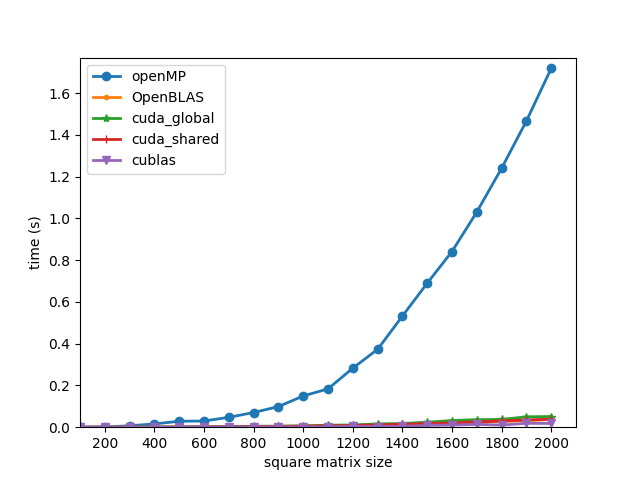
\includegraphics[width=0.8\textwidth]{a2.png}
	\caption{running time of the codes}
	\label{}
\end{figure}
\begin{figure}[H]
	\centering
	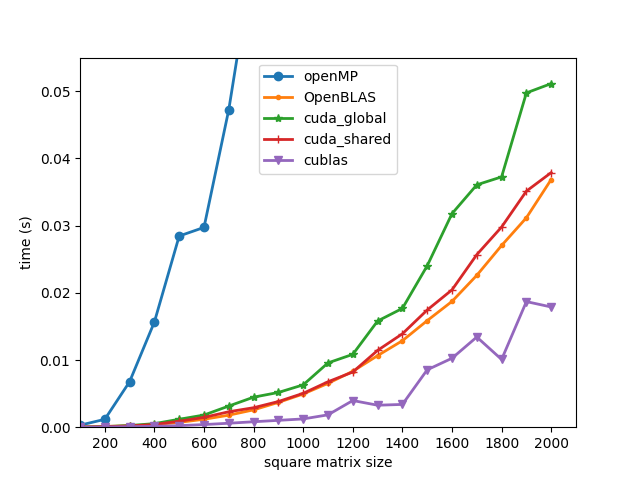
\includegraphics[width=0.8\textwidth]{a.png}
	\caption{running time of the codes with openMP cut}
	\label{}
\end{figure}
Also,their is a GFlops-matrix size version to have a much more intuitive sight.
\begin{figure}[H]
	\centering
	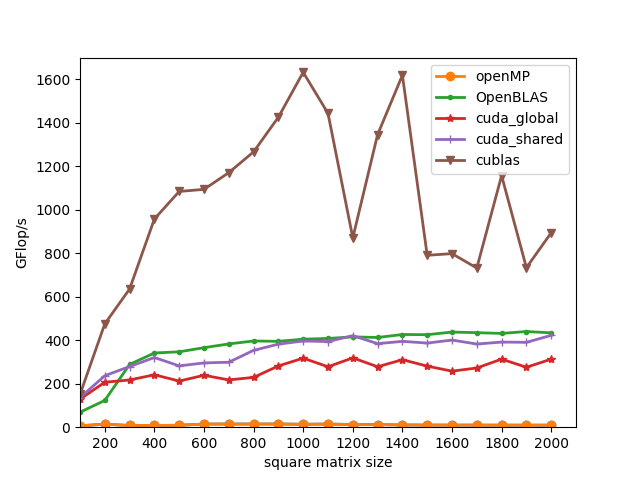
\includegraphics[width=0.8\textwidth]{gflops.png}
	\caption{GFlops performance of the codes}
	\label{}
\end{figure}
It's obvious that the three GPU version are all better than simple CPU parallel openMP version.However the two hand-made GPU version still cannot compare to the openBLAS version,but anyway very close.Only the cuBLAS version leave all the others behind,which might have a great deal of optimization.

Something interesting is that the global memory GPU version is slower than the shared memory GPU version.Since the global memory can be accessed by all the threads both on CPU and GPU,maybe due to hardware restriction,bandwidth or data integrity,the access to this memory will cause race condition.But the shared memory can only be accessed by the block allocated,and do not have race condition problem,thus have better performance.
\end{document}
